\chapter{Overview}

\section*{Introduction}
This introductory chapter presents the general context of the project and gives
an overview of its scope. In the first section, we will specify pedagogical and
professional frame of the project, where we will introduce the host company, its
business field  and the DevOps team. Then, in the second section, we will
present some general concepts of the project. Finally, we will define the
project problematic and present the project goals.

\pagebreak

\section{General context}
In the part we will put the project in its frames, both scholar and
professional. First we will set the pedagogical. Then we will define the
professional frame, i.e Predictix and more specifically the DevOps team.

\subsection{Pedagogical Frame}
This project was elaborated in the context of a graduation internship, a final
step of obtaining the National Diploma of computer engineering from the Faculty
of Science of Tunis.
The internship was undertook on period of four months, from February 1st to May
31th, 2017, during which, we integrated the DevOps team at Predictix Tunisia.
\subsection{Professional frame}

Predictix is an American company headquartered in Atlanta, GA, USA, with a
center of operations in Tunisia.
\subsubsection{Predictix: Foundation and activity domain}

Predictix is a fast growing consulting and software company founded in 2005,
headquartered in Atlanta, Georgia USA with affiliations in Tunis, Tunisia,
London, UK and Amsterdam, Netherlands. It merged with LogicBlox in January 2014
which private company that provide the next generation of smart database. This
new database permits to present finished products to the clients in the simplest
ways, after performing a lot of complicated cloud and multicore computing.

Predictix is specialized in providing software solutions implementing predictive
analytic technologies to solve retail problems and improves retailers'
profitability. In fact, it helps Tier 1 TODO retailers and brands make better
merchandising decisions  by eliminating the traditional silos between varrious
buying and selling decision, delivering solutions that evolve easily to adapt to
their ever-changing business and simplifying the process and lowering the stakes
of investing in technology.

As recognition, Gartner, the world's leading information technology research and
advisory company, has classified as a leader, in the Magic Quadrant for
Merchandise Assortment Management Applications in July 2015.

As a matter fact, because of the leading role of Predictix in Cloud based
solutions for retailers. It get acquired by Infor, in 2016.

\subsubsection{Infor}
Infor is the third-largest provider of enterprise applications and services
behind Oracle and SAP. Think: over 70,000 customers in 194 countries for its
industry-specific applications and suites designed for the cloud, on-premises,
or both, that brings in about \$2.5 billion in revenue. To handle this massive
operation, Infor employs 13,000 people across the globe.

Predictix joined Infor as the base of Infor-retail the Infor division for
retailers.

Infor on Predictix:
"Atlanta-based Predictix experienced more than 40 percent growth in SaaS
subscriptions in 2015 and counts 5 of the top 15 global retailers as customers,
managing more than \$60bn in weekly forecasts. The company has an engineering-
and science-driven culture with deep expertise in retail and a drive to
revolutionize the industry. LogicBlox, the company's technology platform
underlying all Predictix applications, revolutionizes the development of
next-generation predictive and prescriptive applications, and has attracted
funding from DARPA, the Defense Advanced Research Projects Agency."

Predictix is providing SaaS applications to big retailers, among which the
largest drug retail chain in the United States in sales and profits with annual
sales of over US \$76 billion in 2015, employs over 240,000 people, with more
than 8,000 stores  across all 50 U.S States, the District of Columbia, Porto
Rico and the US Virgin Islands. As a matter of act, for forecasting purposes,
this client benefited from \$125M from inventory reduction alone, with 20\% of
ongoing. Some of Predictix clients, whose solutions are already on production,
are
\begin{itemize}
\item{Kiabi}
\item{The Home Depot}
\item{Crate and Barrel}
\item{M.Video}
\item{Target}
\end{itemize}

Predictix offers its clients a variety of solutions. The figure gives an
overview of Predictix business units:

\begin{figure}[h]
  \center
  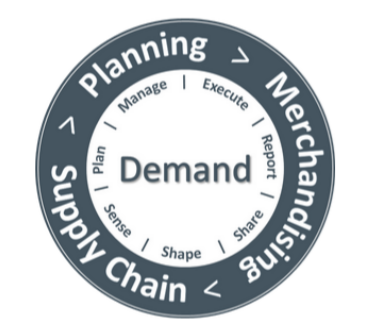
\includegraphics[width=6cm]{planning-supply}
\caption{Merchandising Predictix Suite}
\label{fig:planning-supply}
\end{figure}

Pricing and Promotions: Retailers, wholesalers and some manufacturers use
Predictix services to help them manage their promotions, pricing and markdowns
for higher profit bottom lines,by offering a very high flexible and
configurable solution that facilitates the user interaction with the results he
gets.

\begin{itemize}
\item{\textbf{Forecasting  and Replenishment}: The firm provides forecasts and
    replenishment strategies that enable a retailer to implement the
    promotional, pricing and assortment strategies established. Additional
    profit can be gained by minimizing inventory levels and reducing lost
    sales.}

\item{\textbf{Assortment and Space Optimization}: Predictix helps retailers to
    define the optimal localized assortment for every store and every space.
    Retailers can expect category margins to improve 100 basis points or more,
    and to drive higher sales, from optimizing their assortment with Predictix
    ASO.}
\item{\textbf{Planning and  Allocation}: Business Consulting at Predictix helps
    retailers review their current planning and allocation process and design
    new ones for the future.}
\end{itemize}

\noindent In order to provide these solutions , Predictix has forged a number of
strategic partnerships with other companies. Some of which are the following
companies:

\begin{itemize}
  \item{\textbf{LogicBlox}: The platform provider for Predictix' solutions. Predictix use
LogicBlox' scalable and declarative database system, programming language and
different environment tools to design and build  its systems. After a
partnership lasting for years, the two companies have merged together.}

\item{\textbf{Amazon Web Services}: AWS is a world leader in cloud computing
solutions. Predictix is using AWS' IaaS and PaaS solutions to host its different
systems. The need for cloud services will be detailed later in the next chapter.}
\end{itemize}

During its life cycle, every client's product goes through a number of steps,
from development to testing to deployment. Most of tools and steps of the
development pipeline are the responsibility of the DevOps team within which we
undertook this internship.

\subsubsection{DevOps team}

The DevOps team is needed in every step of the client's product life cycle. In f
fact, they gather and collect the data, store it, do batch processing or
real-time processing on it, and serve it via an API to a data scientist who can
easily query it. They have extensive knowledge on databases and best
engineering practices. These include handling and logging errors, monitoring
the system, building human-fault-tolerant pipelines, understanding what is
necessary to scale up, addressing continuous integration, knowledge of database
administration, maintaining data cleaning and ensuring a deterministic
pipeline.

The main activities of Predictix's architecture and integration team can be
summarized to:

$\bullet$ They intervene, in the beginning of the project when the requirements are
defined. They play the role of consultant as they are consulted to discuss the
data specification, in collaboration with the data science team, with the
client. In fact, their role, at this step is to take all necessary measures in
order to make sure that the data is normalized and consistent.

$\bullet$ They intervene, also, in the development of the applications, as they are in
charge of the applications architecture design. In fact, they translate complex
functional and technical requirements into detailed architecture, design and
high performing software with the ability to architect highly scalable
distributed systems.

$\bullet$ They are, also, in charge of batch implementation thorough data modelling, rules
definitions, protocol buffers services, etc.

$\bullet$ Finally they are responsible of the application being automatically build and
deployed on the cloud, with extremely high attention to the application
performance, as it world affect the application cost.

$\bullet$ One of the main duties of the DevOps team. Is to create internal
tools that facilitate the development of project, deploying and monitoring
performance and cost.

\textbf{lb-job-cost}: It's a tool for monitoring lb jobs cost of each client's account.
It will give the current actual cost for the month along with the projected cost
for the whole month.

\textbf{lb-workflow-console}: It's a web application that helps engineers at Predictix to monitor
the batch process in real-time.

\textbf{Command-history}: A web applications that monitor the commands used in all
Predictix EC2 machines. It give the user the ability to search the history of command
usage.

\textbf{Nixops-dashboard}:
SaaS solution that allows users with no technical knowledge, to easily provision
Predictix applications on the cloud.  Business consultants, testers, and others are
now able to deploy complex infrastructures with a click of button.

\textbf{lamias-servicetester}: A DSL for testing web services. It can be used for unit
tests and for regression tests.

\section{Project presentation}

Since Predictix works with 1 tier retailers in the US, application data tend to
be large enough to face issue in performance. In fact some of Predictix client
deliver weekly data of the size of 2 TB of sales records. 
Developer need to monitor the performance of the application during development
phase.

\subsection{Problematic}
Measuring the performance of an application is an operation that has to be done on
daily basis or every time changes are introduced in the application codebase or
one its dependencies.
To automate the benchmarking process, we need first to understand how developer
are doing benchmarks currently.

\subsubsection{Timing services}
Compare to traditional 3-tired development stack, Business logic is installed in
the LB database itself, Thus simplifying  application development by alleviating
the need for:
\begin{itemize}
\item{Fetching data to and from DB }
\item{Integration between OLAP and OLTP}
\item{Simpler language for business logic}
\end{itemize}

So all LB applications expose a set of services to the client (mostly the UI).
Each service is a feature in the application or a part of a feature. To test the
performance we measure the time it took for a request to one of the services to
complete, Thus measuring both the performance of the application and the
LogicBlox database.

The services request are predefined as Lamias tests. The tests can be Relax
query or simple HTTP requests. The definition of the Lamias tests used in the
benchmarks differ per application. Thus benchmarking is only relevant in the
scope of one application. Thus, benchmarks of different application can't be
used to compare the performance of the two. Also the tests used to measure the
performance of one application can't be reused in the benchmark of another one.

\section*{Conclusion}
The first chapter provided an overview of the general context of the project and
its scope. We introduced the host company and the technical DevOps along with
project problematic.
